\documentclass{standalone}
\usepackage{tikz}
\usepackage{amsmath}
\usepackage{color}
\usetikzlibrary{matrix}
\usetikzlibrary {shapes.geometric}
\usetikzlibrary {math}
\usetikzlibrary {arrows.meta}

\begin{document}
        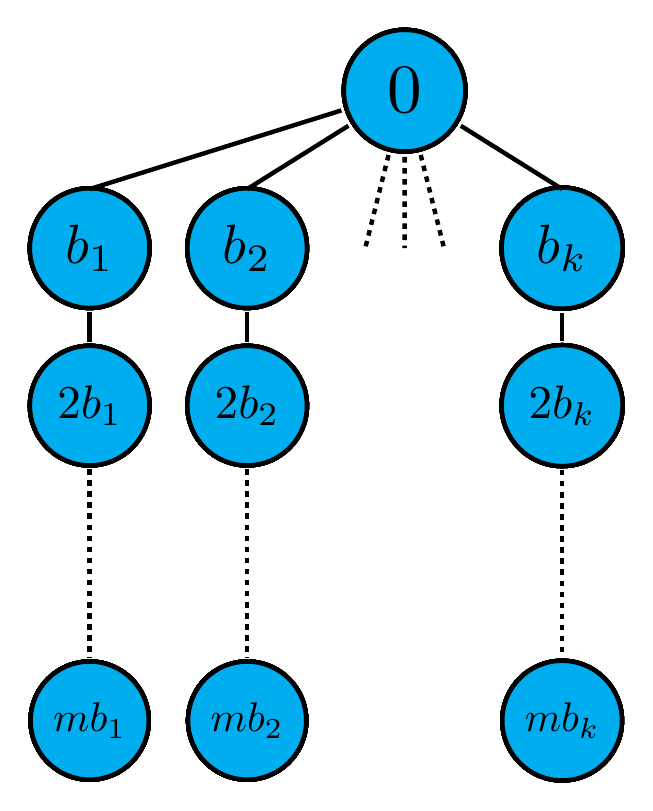
\begin{tikzpicture}
        %    \draw [help lines] (0,0) grid (16,16);
        \foreach \x/\y in {1,2,4,6,8/1,2,4,6,8,10}
        {
            \draw [fill=cyan] (6,10) circle [radius=0.77]  ;
            \path node (a) [ultra thick,circle,draw,scale = 2.5]at (6,10) {0};

            \draw [fill=cyan] (2,8) circle [radius=0.77]  ;
            \path node (b) [ultra thick,circle,draw,scale = 2]at (2,8) {$b_{1}$};
           
            \draw [fill=cyan] (4,8) circle [radius=0.77]  ;
            \path node (c) [ultra thick,circle,draw,scale = 2]at (4,8) {$b_{2}$};
            
            \draw [fill=cyan] (8,8) circle [radius=0.77]  ;
            \path node (d) [ultra thick,circle,draw,scale = 2]at (8,8) {$b_{k}$};
            
            \draw [fill=cyan] (2,6) circle [radius=0.77]  ;
            \path node (e) [ultra thick,circle,draw,scale = 1.7]at (2,6) {$2b_{1}$};

            \draw [fill=cyan] (4,6) circle [radius=0.77]  ;
            \path node (f) [ultra thick,circle,draw,scale = 1.7]at (4,6) {$2b_{2}$};

            \draw [fill=cyan] (8,6) circle [radius=0.77]  ;
            \path node (g) [ultra thick,circle,draw,scale = 1.7]at (8,6) {$2b_{k}$};

            \draw [fill=cyan] (2,2) circle [radius=0.77]  ;
            \path node (h) [ultra thick,circle,draw,scale = 1.5]at (2,2) {$mb_{1}$};

            \draw [fill=cyan] (4,2) circle [radius=0.77]  ;
            \path node (i) [ultra thick,circle,draw,scale = 1.5]at (4,2) {$mb_{2}$};

            \draw [fill=cyan] (8,2) circle [radius=0.77]  ;
            \path node (j) [ultra thick,circle,draw,scale = 1.5]at (8,2) {$mb_{k}$};
        }

       
        \draw[ultra thick] [dash pattern=on 2pt off 2pt](a) -- (5.5,8);
        \draw[ultra thick] [dash pattern=on 2pt off 2pt](a) -- (6,8);  
        \draw[ultra thick] [dash pattern=on 2pt off 2pt](a) -- (6.5,8);    
       
        \draw[ultra thick] (a) -- (2,8.75); 
        \draw[ultra thick] (a) -- (4,8.75); 
        \draw[ultra thick] (a) -- (8,8.75); 

        \draw[ultra thick] [dash pattern=on 2pt off 2pt](e) -- (h); 
        \draw[ultra thick] [dash pattern=on 2pt off 2pt](f) -- (i); 
        \draw[ultra thick] [dash pattern=on 2pt off 2pt](g) -- (j); 

        \draw[ultra thick] (b) -- (e); 
        \draw[ultra thick] (c) -- (f); 
        \draw[ultra thick] (d) -- (g); 
        
        
         
    
    \end{tikzpicture}
\end{document}